\section{Simulations}

\subsection{Characteristics of the system}

To verify the results in practice, a SIMULINK model was created whose step response resembles the one of the experimental setup as close as possible.

In Figure \ref{fig:block_dia_simu} the blockdiagram of the system can be observed. It's step response is depicted in Figure \ref{fig:step_resp_simu}

\begin{figure}[H]
\begin{center}
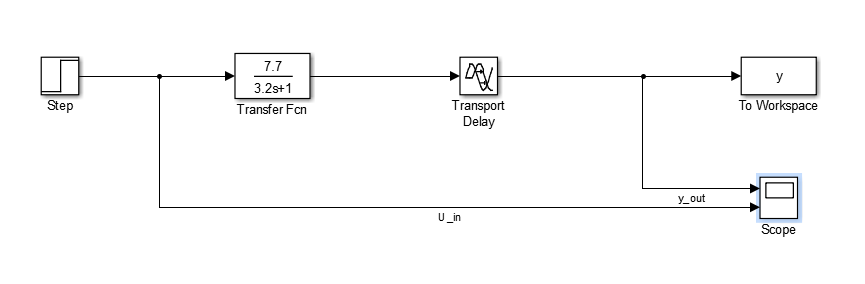
\includegraphics[width=1\linewidth]{images/general/block_dia_simu}
\end{center}
\caption{Block diagram of the simulation}
\label{fig:block_dia_simu}
\end{figure}

\begin{figure}[H]
\begin{center}
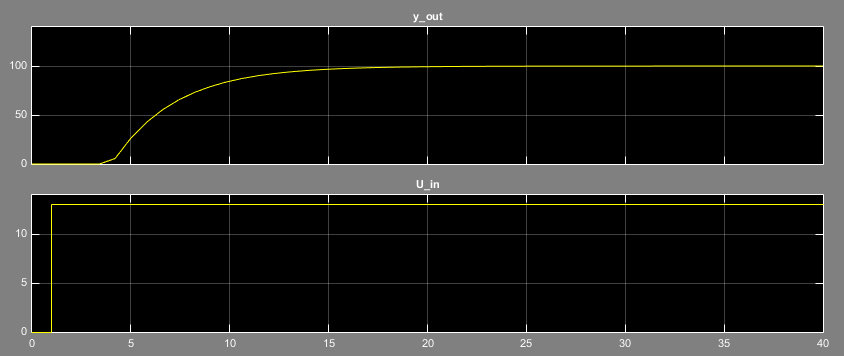
\includegraphics[width=1\linewidth]{images/general/step_resp_simu}
\end{center}
\caption{Step response the system}
\label{fig:step_resp_simu}
\end{figure}

\subsection{Controlling the system}

After the system was close enough to the one form the experimental setup, a PID controller was added according to Figure \ref{fig:PID_system}. At first the output started to raise to infinity very quickly, using the PID parameters determined in the experimental setup. One problem was that the error fed into the PID-Controller was in units of rpm whilst the input to the system was expected in volts. Then a saturation limitter was added to have the maximum output of the PID-Controller be max [-13, 13]. The PID-Controller then behaved nicely as seen in Figure \ref{fig:system_control1}. Unfortunately it misses the setpoint by 10 percent. All tries to make this behaviour better were a failure. Tinkering with the tuning function of MATLAB produced much better results as seen in Figure \ref{fig:system_control2}. It seems like the integrator part of the PID values is way too high from the value gained in the experiments and the integrator of the MATLAB PID controller gets to a point of no return where it will always strive to gain even more which is why the system stays at it's upper limit.

The final MATLAB-tuned PID values can be obtained from Table \ref{tab:final_values}.

\begin{table}[H]
\begin{center}
\begin{tabular}{ l | r}
  Parameter & Value\\
  \hline
  \hline
  $K_p$ & $0.0566$\\
  \hline
  $T_i$ & $0.0171$\\
  \hline
  $T_d$ & $0$\\
  \hline
\end{tabular}
\end{center}
\caption{Final MATLAB-tuned PID values}
\label{tab:final_values}
\end{table}

\begin{figure}[H]
\begin{center}
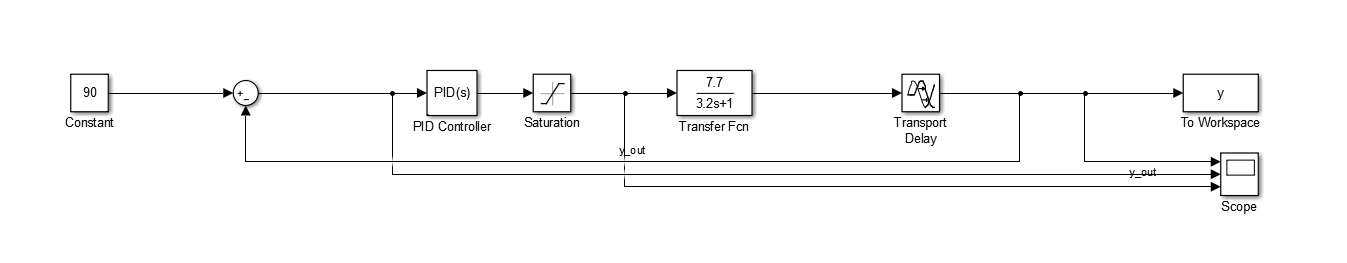
\includegraphics[width=1\linewidth]{images/general/PID_system}
\end{center}
\caption{The simulation system with a PID-Controller added}
\label{fig:PID_system}
\end{figure}

\begin{figure}[H]
\begin{center}
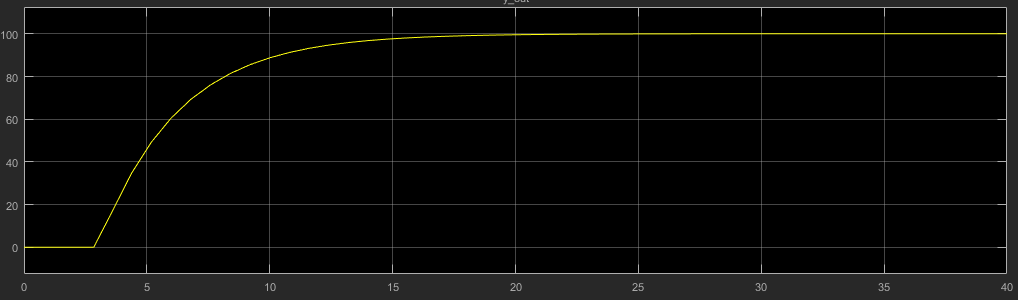
\includegraphics[width=1\linewidth]{images/general/system_control1}
\end{center}
\caption{Behavior of the system controlled by the experimental controller}
\label{fig:system_control1}
\end{figure}

\begin{figure}[H]
\begin{center}
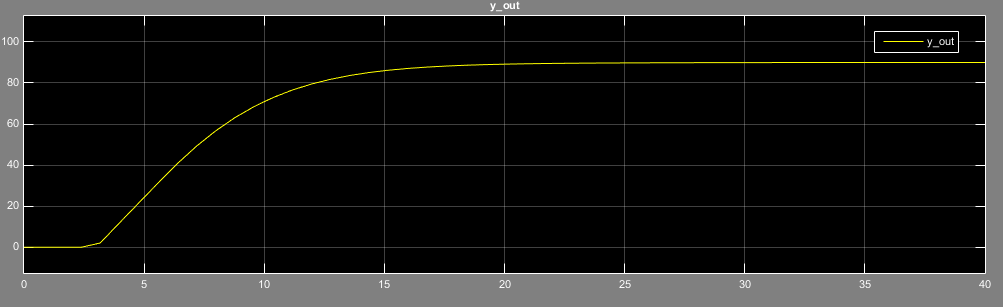
\includegraphics[width=1\linewidth]{images/general/system_control2}
\end{center}
\caption{Behavior of the MATLAB-tuned, controlled system}
\label{fig:system_control2}
\end{figure}
\newpage
